\documentclass{article}

\usepackage{booktabs, amssymb, amsfonts, float}
\usepackage{mathtools}
\usepackage{enumitem}
\usepackage{geometry}
\geometry{margin=1in}
\usepackage{graphicx} 
\usepackage{booktabs} 
\usepackage{listings}
\usepackage{xcolor}

\lstdefinestyle{mystyle}{
    backgroundcolor=\color{white},
    commentstyle=\color{gray},
    keywordstyle=\color{blue},
    numberstyle=\tiny\color{gray},
    stringstyle=\color{orange},
    basicstyle=\ttfamily\footnotesize,
    breaklines=true,                 
    captionpos=b,
    keepspaces=true,                 
    numbers=left,                    
    numbersep=5pt,                  
    showspaces=false,                
    showstringspaces=false,
    showtabs=false,                  
    tabsize=2
}
\lstset{style=mystyle}

\usepackage{tikz}
\usetikzlibrary{
  arrows.meta,
  positioning,
  shapes.geometric,
  calc,
  fit,
  backgrounds,
  decorations.pathreplacing
}

\title{Token-Adaptive Gated Attention Transformer}

\author{
  Shreel Golwala \\
  Virginia Tech \\
  \texttt{golwalas@vt.edu}
}

\date{}
\begin{document}
\maketitle
\section{Abstract}
\noindent
Transformers have set the standard for modeling long-range dependencies in language and multimodal tasks, but traditional architectures apply the same computations to all tokens. A modular Transformer is introduced that combines sparse gated routing with per-token FiLM-style modulation. The architecture consists of multiple expert modules, each a complete multi-head self-attention block with its own feedforward network. A learned gating network selects a sparse subset of experts for each token, creating individualized processing paths, while token-specific FiLM parameters dynamically modulate expert outputs without altering the base attention weights. Balanced and specialized routing is explored on the MultiNLI dataset, showing that even expert utilization improves generalization, while specialization allows experts to capture fine-grained linguistic patterns. Compared to a vanilla Transformer tested under the same conditions, the modular Transformer achieves a mean validation accuracy of 0.6333 (std $\approx$ 0.0482), peaking at 0.6720 versus 0.5185 $\pm$ 0.0238 for the baseline, with training accuracy of 0.9338 versus 0.5881. This proposed model produces a more expressive and flexible architecture that captures token-level nuances more effectively, resulting in higher accuracy and stronger performance.


\section{Introduction and Background}

\subsection{Self-Attention in Transformers}
Transformers have become the foundation of modern deep learning architectures in language, vision, and multimodal tasks, due to their ability to model long-range dependencies via self-attention mechanisms\textsuperscript{[1]}. Given an input sequence of token embeddings $X = [x_1, x_2, \ldots, x_T]$, the self-attention layer computes contextual representations by forming queries, keys, and values as:
\[
Q = X W_Q, \quad K = X W_K, \quad V = X W_V,
\]
where $W_Q, W_K, W_V \in \mathbb{R}^{d \times d}$ are learned projection matrices. The attention scores are computed using scaled dot-product attention:
\[
\text{Attention}(Q, K, V) = \text{softmax} \left( \frac{Q K^\top}{\sqrt{d}} \right) V.
\]


\noindent
This mechanism allows each token to aggregate information from all others in the sequence, giving it a unique, context-aware understanding.

\subsection{Limitations of Standard Transformers}

In standard Transformers, all tokens pass through the same sequence of layers, each consisting of shared attention and feedforward blocks (FFNs). There is no notion of routing or token-specific parameterization:

\begin{itemize}
    \item Each token receives the same computation, regardless of its semantics. 
    \item Attention is applied uniformly across all heads and tokens. 
    \item The model does not modulate internal computations based on token difficulty, syntactic role, or other related factors. 
\end{itemize}

\noindent
This one-size-fits-all processing can be inefficient or suboptimal for heterogeneous inputs with varying structural complexity, where some tokens require deep contextual modeling, while others may not.


\subsection{Mixture-of-Experts: Routing Without Modulation}

\vspace{4pt}
Mixture-of-Experts (MoE) architectures address this by introducing conditional computation. Instead of applying a uniform transformation to all tokens, MoE uses a gating/routing network to selectively activate a sparse subset of $N$ experts $\{M_1, \ldots, M_N\}$ for each token\textsuperscript{[2, 3]}. Each expert specializes in a different computational behavior. For a token representation $x_t$, the gating network computes a score vector:
\[
g_t = W_g x_t + b_g, \quad g_t \in \mathbb{R}^N,
\]
where \( W_g \) is the learned routing matrix that determines how the input features influence the selection of the expert, \( g_t \) contains a score for each expert and represents how suitable that expert is for processing a token \( x_t \), and \( b_g \) is the bias term.


\noindent
This is followed by sparse selection of the top-$k$ experts (higher the score, more likely that expert will be selected):
\[
{E}_t = \text{TopK}(g_t, k),
\]
and a softmax over selected logits to normalize into positive weights that sum to 1:
\[
\tilde{g}_t^{(i)} = \frac{\exp(g_t^{(i)})}{\sum_{j \in {E}_t} \exp(g_t^{(j)})}, \quad i \in {E}_t.
\]
This allows for sparsity and specialization --- each token activates only a few expert modules. 

\subsection{Limitations of MoEs}
However, traditional MoE experts are typically simple feedforward MLPs with no attention or internal adaptation. Thus: 
\begin{itemize}
    \item MoEs prioritize scalability but lack expressivity as MLP-based experts may be insufficient for modeling complex dependencies and contextual reasoning.
    \item Expert behavior is static; it does not adapt per token beyond the gating choice. 
    
\end{itemize}


\noindent
These shortcomings limit their usefulness in NLP settings that demand both efficiency and token-level adaptability. 

\subsection{FiLM Modulation}

Meta-learning techniques such as Feature-wise Linear Modulation (FiLM)\textsuperscript{[4]} offer a mechanism for dynamic adaptation. A lightweight meta-network generates per-token modulation parameters \((\gamma_t, \beta_t)\), which can alter the behavior of internal modules conditioned on the input itself:
\[
\hat{h}_t = \gamma_t \odot h_t + \beta_t, \quad \gamma_t, \beta_t \in \mathbb{R}^d.
\]

\noindent
Both parameters are learned via backpropagation, letting the meta-network highlight or suppress features based on token context. When applied to expert modules, this allows each expert to adapt its behavior per token, boosting expressivity without increasing depth or parameter count. 




\vspace{3pt}



\section{Overview}
In this work, a modular transformer architecture is introduced that applies gated sparse routing over full attention-based expert modules, where each expert is a complete multi-head self-attention (MHSA) block. A learned gating network selects a sparse subset of experts for each token, allowing for conditional computation along token-specific pathways. To further improve expressiveness, each expert output is modulated by token-specific meta-parameters generated by a lightweight FiLM-style meta-network. This creates a layered system in which each token not only selects which attention modules to use, but also how those modules process the token—which gives structural diversity and dynamic flexibility.
\vspace{3pt}



\section{Architecture}

\subsection{Input Representation}

Let the input sequence be 
\[
X = [x_1, x_2, \dots, x_T], \quad x_t \in \mathcal{V}
\]
where \( \mathcal{V} \) is the vocabulary set. Each token \( x_t \) is a word or subword unit drawn from this vocabulary. Tokens are embedded using a learned embedding matrix, \( \text{Embed}: \mathcal{V} \to \mathbb{R}^d \), such that:

\[
e_t = \text{Embed}(x_t) \in \mathbb{R}^d
\]

\noindent
Collecting all token embeddings results in:

\[
E = [e_1, e_2, \dots, e_T] \in \mathbb{R}^{T \times d}
\]


\noindent
To retain positional information, the fixed sinusoidal or learned positional encodings \( P \in \mathbb{R}^{T \times d} \) are added, producing the initial input to the transformer:

\[
H^{(0)} = E + P
\]

\subsection{Gating Network and Sparse Routing}

At each transformer layer \( \ell \), the token embedding \( h_t^{(\ell)} \in \mathbb{R}^d \) is passed through a linear transformation to compute expert selection scores:

\[
g_t = W_g h_t^{(\ell)} + b_g, \quad g_t \in \mathbb{R}^N
\]


\noindent
where \( W_g \in \mathbb{R}^{N \times d} \), \( b_g \in \mathbb{R}^N \), and \( N \) is the number of experts. We select the top-\( k \) experts with the highest scores:

\[
E_t = \text{TopK}(g_t, k)
\]


\noindent
To compute differentiable expert weights, the sparse softmax is applied over the selected experts \( E_t \):

\[
\tilde{g}_t^{(i)} = \frac{\exp(g_t^{(i)})}{\sum_{j \in E_t} \exp(g_t^{(j)})}, \quad i \in E_t
\]


\noindent
This gives a confidence distribution over the top-k experts for each token.

\subsection{Attention-Based Expert Modules}

Each expert \( M_i \) is implemented as a Transformer block with Multi-Head Self-Attention (MHSA). For each attention head \( h \in \{1, \dots, H\} \), and hidden dimension \( d_h = \frac{d}{H} \), we compute:

\[
Q_t^{(i,h)} = W_{Q,i}^{(h)} h_t^{(\ell)}, \quad 
K_j^{(i,h)} = W_{K,i}^{(h)} h_j^{(\ell)}, \quad 
V_j^{(i,h)} = W_{V,i}^{(h)} h_j^{(\ell)}
\]


\noindent
where \( W_{Q,i}^{(h)}, W_{K,i}^{(h)}, W_{V,i}^{(h)} \in \mathbb{R}^{d \times d_h} \) are expert- and head-specific weight matrices (Query, Key, Value). The scaled dot-product attention is then:

\[
\alpha_{tj}^{(i,h)} = \frac{\exp \left( \frac{Q_t^{(i,h)\top} K_j^{(i,h)}}{\sqrt{d_h}} \right)}{\sum_{m=1}^{T} \exp \left( \frac{Q_t^{(i,h)\top} K_m^{(i,h)}}{\sqrt{d_h}} \right)}
\]


\noindent
The output for head \( h \) is a weighted sum over all positions:

\[
O_t^{(i,h)} = \sum_{j=1}^{T} \alpha_{tj}^{(i,h)} V_j^{(i,h)}
\]


\noindent
The final output of expert \( M_i \) for token \( t \) is calculated by concatenating outputs from all heads:

\[
M_i(h_t^{(\ell)}) = \text{Concat}(O_t^{(i,1)}, \dots, O_t^{(i,H)}) \in \mathbb{R}^d
\]

\subsection{Meta-Adaptation via FiLM}

To enable expert outputs to dynamically adapt to each token, we apply FiLM (Feature-wise Linear Modulation). A meta-network \( \text{Meta}_i \) produces scale and shift vectors for each expert and token:

\[
[\gamma_t^{(i)}, \beta_t^{(i)}] = \text{Meta}_i(h_t^{(\ell)}), \quad \gamma_t^{(i)}, \beta_t^{(i)} \in \mathbb{R}^d
\]


\noindent
These are applied elementwise to modulate the expert outputs:

\[
\hat{M}_i(h_t^{(\ell)}) = \gamma_t^{(i)} \odot M_i(h_t^{(\ell)}) + \beta_t^{(i)}
\]

\subsection{Aggregation of Expert Outputs}

The final representation for each token is a weighted sum over the modulated outputs of the selected experts:

\[
y_t^{(\ell+1)} = \sum_{i \in E_t} \tilde{g}_t^{(i)} \cdot \hat{M}_i(h_t^{(\ell)})
\]


\noindent
This is followed by a residual connection (for gradient flow) and layer normalization (stabilize outputs):

\[
h_t^{(\ell+1)} = \text{LayerNorm}(h_t^{(\ell)} + y_t^{(\ell+1)})
\]

\subsection{Training Objective}

\subsubsection{Task Loss (Cross Entropy)}

The main supervised loss for prediction is:

\[
\mathcal{L}_{\text{task}} = \frac{1}{T} \sum_{t=1}^{T} \ell(\hat{y}_t, y_t^{\text{true}})
\]

where \( \hat{y}_t \) is the model output and \( y_t^{\text{true}} \) is the ground truth.

\subsubsection{Routing Entropy-Based Loss}

To encourage confident, sparse expert selection by examining the routing probabilities for each token during routing:

\[
H_t = -\sum_{i \in E_t} \tilde{g}_t^{(i)} \log \tilde{g}_t^{(i)}, \quad \mathcal{L}_{\text{entropy}} = \frac{1}{T} \sum_{t=1}^{T} H_t
\]

\subsubsection{L2 Load Balancing Loss}

To prevent expert underutilization, the distribution of routing weights are regularized/penalized by checking the assignments after all tokens have been routed:

\[
u_i = \frac{1}{T} \sum_{t=1}^{T} \tilde{g}_t^{(i)}, \quad 
\mathcal{L}_{\text{balance}} = \sum_{i=1}^{N} \left( u_i - \frac{1}{N} \right)^2
\]

\subsubsection{Total Loss}

The total training loss combines all objectives:

\[
\mathcal{L} = \mathcal{L}_{\text{task}} + \lambda_1 \mathcal{L}_{\text{entropy}} + \lambda_2 \mathcal{L}_{\text{balance}}
\]


\noindent
where \( \lambda_1, \lambda_2 \) are hyperparameters controlling tradeoffs.

\vspace{5pt}
\begin{figure}[ht!]
    \centering
    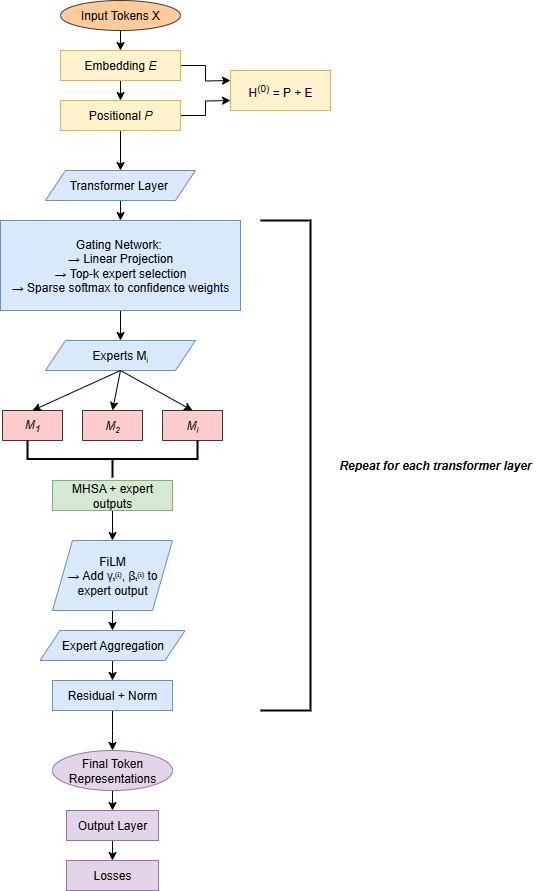
\includegraphics[width=0.4\linewidth]{gmat_final_arc.drawio.png}
    \caption{Architecture flow}
    \label{fig:arc_flow}
\end{figure}

\section{Code Implementation}

All code segments are simplified for clarity and understanding\footnote{https://github.com/shreelg/TAGAT}. 

\subsection{Configuration-Driven Initialization}


All model and training hyperparameters are stored in a centralized configuration object (\texttt{Config}), which is passed to all submodules (Embedding, Expert, Gating, MetaFiLM) at construction to keep setup consistency and simplify modifications.
\vspace{3pt}

\begin{lstlisting}[language=Python, caption={ \texttt{Config} object (Specific parameter values may vary per experiment)}, label={lst:config}]
class Config:
    vocab_size = 30522
    d_model = 128
    num_heads = 4
    num_experts = 4
    top_k = 2
    num_layers = 1
    max_seq_len = 128
    batch_size = 32
    num_classes = 2
    lr = 1e-4
    lambda_entropy = 1e-2
    lambda_balance = 1e-2
    device = 'cuda' if torch.cuda.is_available() else 'cpu'

config = Config()
\end{lstlisting}



\subsection{Input Encoding Module}
The input encoder consists of a \texttt{TokenEmbedding} layer implemented via \texttt{nn.Embedding}, combined with a \texttt{PositionalEncoding} component, either sinusoidal (deterministic) or learned (parameterized). These are composed into a unified \texttt{TokenEncoder} class, producing the initial representation tensor:
\[
X^{(0)} \in \mathbb{R}^{B \times T \times d_{\mathrm{model}}}
\]
for a batch of size $B$ and sequence length $T$.
This tensor is the input to the first Gated Modular Layer, combining token and positional embeddings to provide spatial and semantic information from the start.
\vspace{3pt}

\begin{lstlisting}[language=Python, caption={\texttt{TokenEncoder} module}, label={lst:input_enc}]
class TokenEncoder(nn.Module):
    def __init__(self, config):
        super().__init__()
        #Embedding layer
        self.token_embed = nn.Embedding(config.vocab_size, config.d_model)

        #Positional encoding 
        positions = torch.arange(config.max_seq_len).unsqueeze(1)
        div_term = torch.exp(torch.arange(0, config.d_model, 2) *
                             (-math.log(10000.0) / config.d_model))
        pe = torch.zeros(config.max_seq_len, config.d_model)
        pe[:, 0::2] = torch.sin(positions * div_term)
        pe[:, 1::2] = torch.cos(positions * div_term)

        self.register_buffer("pos_enc", pe.unsqueeze(0))  # (1, T, d_model)

    def forward(self, input_ids):
        x = self.token_embed(input_ids)                   # (B, T, d_model)
        return x + self.pos_enc[:, :x.size(1)]            # Add embedding + positional


\end{lstlisting}




\subsection{Expert Submodules}
Each expert is implemented as an \texttt{Expert} class containing:
\begin{itemize}
    \item Multi-Head Self-Attention (MHSA) with residual connections, allowing token-to-token interactions within the expert’s processing context.
    \item Position-wise Feedforward Network (FFN) consisting of two linear layers with ReLU activation and dropout.
    \item Layer normalization applied after both MHSA and FFN to stabilize training and decouple layer statistics.
\end{itemize}
All experts are stored in an indexed \texttt{ModuleList} which allows direct retrieval based on runtime routing decisions and is essential for efficient sparse dispatch.
\vspace{3pt}

\begin{lstlisting}[language=Python, caption={\texttt{Expert} module \& container}, label={lst:expert}]
class Expert(nn.Module):
    def __init__(self, config):
        super().__init__()
        # MHSA
        self.self_attn = nn.MultiheadAttention(
            embed_dim=config.d_model,
            num_heads=config.num_heads,
            batch_first=True
        )
        # FFN
        self.ffn = nn.Sequential(
            nn.Linear(config.d_model, config.d_model * 4),
            nn.ReLU(),
            nn.Dropout(0.1),
            nn.Linear(config.d_model * 4, config.d_model),
            nn.Dropout(0.1)
        )
        # Layer normalization 
        self.norm1 = nn.LayerNorm(config.d_model)
        self.norm2 = nn.LayerNorm(config.d_model)

    def forward(self, x, attn_mask=None):
        attn_out, _ = self.self_attn(x, x, x, attn_mask=attn_mask)
        x = self.norm1(x + attn_out)
        ffn_out = self.ffn(x)
        x = self.norm2(x + ffn_out)
        return x

# ModuleList
experts = nn.ModuleList([Expert(config) for _ in range(config.num_experts)])

\end{lstlisting}



\subsection{Sparse Gating Logic}
Routing is implemented in the \texttt{ExpertRouter} module:
\begin{enumerate}
    \item {Logit Projection:} Each token representation $x_t$ is projected to $\mathbb{R}^{n_{\mathrm{experts}}}$.
    \item {Sparse Selection:} The top-$k$ logits are retained via \texttt{torch.topk}.
    \item {Normalized Weights:} Selected logits are passed through a softmax to yield routing weights $\alpha_{t,j}$ for expert $j$ and token $t$.
    \item {Routing Diagnostics:} Entropy of $\alpha_{t,:}$ and expert load statistics are computed for regularization and interpretability.
\end{enumerate}
The router outputs expert indices, associated routing weights, and auxiliary statistics required for downstream diagnostics and regularization losses.

\vspace{3pt}
\begin{lstlisting}[language=Python, caption={Sparse gating/routing}, label={lst:sparse_gate}]
class ExpertRouter(nn.Module):
    def __init__(self, config):
        super().__init__()
        self.top_k = config.top_k
        self.gate = nn.Linear(config.d_model, config.num_experts)

    def forward(self, x):
        logits = self.gate(x)                           # Logit projection
        topk_vals, topk_idx = torch.topk(logits, self.top_k, dim=-1)  # Sparse selection
        weights = F.softmax(topk_vals, dim=-1)          # Normalized weights
        return topk_idx, weights

\end{lstlisting}




\subsection{FiLM Modulation}
To support fine-grained, token-specific adaptation, the \texttt{FiLMModulator} module predicts per-token scaling ($\gamma_t$) and shifting ($\beta_t$) parameters. After each expert processes a token, the output (\(y_t\)) is modulated as:
\[
y_t \leftarrow \gamma_t \odot y_t + \beta_t
\]
where $\odot$ denotes elementwise multiplication. This preserves the expert’s learned transformation while dynamically conditioning it in token context, without altering the expert's weights.

\vspace{3pt}
\begin{lstlisting}[language=Python, caption=\texttt{FiLMModulator} module, label={lst:film}]
class FiLMModulator(nn.Module):
    def __init__(self, config):
        super().__init__()
        self.config = config
        self.film_layer = nn.Linear(config.d_model, 2 * config.d_model) 

    def forward(self, x, cond):
        gamma_beta = self.film_layer(cond) 
        # Linear layer outputs tensor with last dimension 2 * d_model (gamma and beta concatenated)
        gamma, beta = gamma_beta.chunk(2, dim=-1) 

        # Split the tensor into gamma and beta, each of shape [batch_size, seq_len, d_model]
        gamma = gamma.unsqueeze(1)
        beta = beta.unsqueeze(1)
        
        return gamma * x + beta # Modulating expert output
\end{lstlisting}




\subsection{Gated Modular Processing Layer}
The \texttt{GatedModularLayer} orchestrates the complete expert routing and processing sequence:
\begin{enumerate}
    \item Token routing via \texttt{ExpertRouter}.
    \item Dispatching tokens to selected experts.
    \item Expert computation in parallel for each selected expert.
    \item FiLM Modulation through \texttt{MetaFiLM}.
    \item Aggregation of weighted expert outputs.
    \item Residual addition and normalization.
\end{enumerate}

\vspace{3pt}
\begin{lstlisting}[language=Python, caption=GML module, label={lst:gml}]
class GatedModularLayer(nn.Module):
    def __init__(self, config, experts, router, film_modulator=None):
        super().__init__()
        self.config = config
        self.experts = experts
        self.router = router
        self.film_modulator = film_modulator
        self.norm = nn.LayerNorm(config.d_model)

    def forward(self, x, cond=None):
        residual = x  # Save input for residual connection
        topk_idx, weights, diagnostics = self.router(x)  # Route tokens to experts
        outputs = torch.zeros_like(x)  # Initialize output tensor

        for i in range(self.config.top_k):
            expert_ids, expert_weights = topk_idx[..., i], weights[..., i]
            for eid in range(self.config.num_experts):
                mask = (expert_ids == eid)  # Tokens assigned to current expert
                if not mask.any():
                    continue

                expert_out = self.experts[eid](x[mask])  # Expert computation
                if self.film_modulator and cond is not None:
                    # Apply FiLM modulation conditioned on external input
                    expert_out = self.film_modulator(
                        expert_out.unsqueeze(1), cond[mask.any(-1)]
                    ).squeeze(1)

                # Scale by gating weight and accumulate
                outputs[mask] += expert_out * expert_weights[mask].unsqueeze(-1)

        # Residual connection and layer normalization
        return self.norm(outputs + residual), diagnostics
 LayerNorm
        x = self.norm(outputs + residual)

        return x, diagnostics

\end{lstlisting}


\subsection{Multi-Layer Transformer Composition}
The \texttt{GatedModularTransformer} is composed of a stack of \texttt{GatedModularLayer} instances. Each layer processes token representations independently and conditionally based on the routing decisions. The final hidden state of a designated special token (e.g. [CLS]) is forwarded to the classification head.

\vspace{3pt}
\begin{lstlisting}[language=Python, caption=GMT module., label={lst:gmt}]
class GatedModularTransformer(nn.Module):
    def __init__(self, config):
        super().__init__()
        #Pre-trained tokenizer
        self.tokenizer = AutoTokenizer.from_pretrained('bert-base-uncased')
        self.embed = nn.Embedding(config.vocab_size, config.d_model)
        self.pos_enc = PositionalEncoding(config.d_model, config.max_seq_len)
        #Creating multiple GatedModularLayers instances
        self.layers = nn.ModuleList([GatedModularLayer(config) for _ in range(config.num_layers)])
        self.fc_out = nn.Linear(config.d_model, config.num_classes)
    
    def forward(self, input_ids, return_gate_probs=False):
        x = self.embed(input_ids)
        x = self.pos_enc(x)
        total_entropy = 0
        balances = []
        gate_probs = None

        for i, layer in enumerate(self.layers):
        #Gating probabilities 
            if return_gate_probs and i == 0:
                x, entropy, balance, gate_probs = layer(x, return_gate_probs=True)
            else:
                x, entropy, balance = layer(x)
            total_entropy += entropy
            balances.append(balance)

        out = self.fc_out(x[:, 0])
        if return_gate_probs:
            return out, total_entropy, balances, gate_probs
        return out, total_entropy, balances
\end{lstlisting}


\subsection{Output Head}
The \texttt{ClassificationHead} applies dropout to the final [CLS] token embedding and projects it to task-specific logits via a linear transformation:
\[
z = W_{\mathrm{out}} \cdot h_{[\mathrm{CLS}]} + b_{\mathrm{out}}
\]
This head can be replaced with regression or multi-task output modules without modifying upstream layers.

\vspace{3pt}
\begin{lstlisting}[language=Python, caption=\texttt{x[:, 0]} is the final token embedding., label={lst:output}]
out = self.fc_out(x[:, 0])
\end{lstlisting}


\subsection{Loss Functions and Metric Logging}
The \texttt{LossManager} aggregates multiple objectives:
\begin{itemize}
    \item Cross-entropy.
    \item Entropy regularization.
    \item Load balancing loss.
\end{itemize}
During training and validation, metrics such as accuracy, macro-F1, routing entropy, and expert load imbalance are logged for later analysis. For visualization, heatmaps, histograms of parameters, and plots of expert usage are also created. 

\vspace{3pt}
\begin{lstlisting}[language=Python, caption=Loss calculations, label={lst:loss}]
logits, entropy, balance = model(input_ids)

loss_cls = ce_loss(logits, labels) 
avg_balance = torch.stack(balance).mean(dim=0)
loss_balance = ((avg_balance - 1 / config.num_experts) ** 2).sum()

regularization + load balancing
loss = loss_cls + config.lambda_entropy * entropy + config.lambda_balance * loss_balance
\end{lstlisting}


\subsection{Training \& Inference Loop}
Data ingestion leverages \texttt{Bert-Base-Uncased} model for tokenization. Dynamic padding and collation use a custom \texttt{collate\_fn} to minimize padding and maximize GPU efficiency.
Inference runs in \texttt{eval} mode with gradients off to save memory and speed up computation. All training and inference were performed on a NVIDIA T4 GPU. 


\section{Experiments}

\subsection{MultiNLI Benchmark}
The proposed architecture is compared against a vanilla Transformer, a standard implementation without any modifications, serving as the baseline model. Both models were trained on MultiNLI, a large reasoning/entailment dataset, for 20 epochs with validation after each epoch. To evaluate the overall efficiency of the proposed model, two configurations were used: a balanced expert usage setup with $\lambda_\text{entropy} = 2$ and $\lambda_\text{balance} = 3$, and a specialized setup with $\lambda_\text{entropy} = 1$ and $\lambda_\text{balance} = 1$. Training used batch size of 64, full data, top-$k = 2$, 4 experts, 4 heads, sequence length 128, and learning rate $1 \times 10^{-4}$.

\noindent
\subsubsection{Balanced Proposed Model}


\begin{figure}[H]
    \centering
    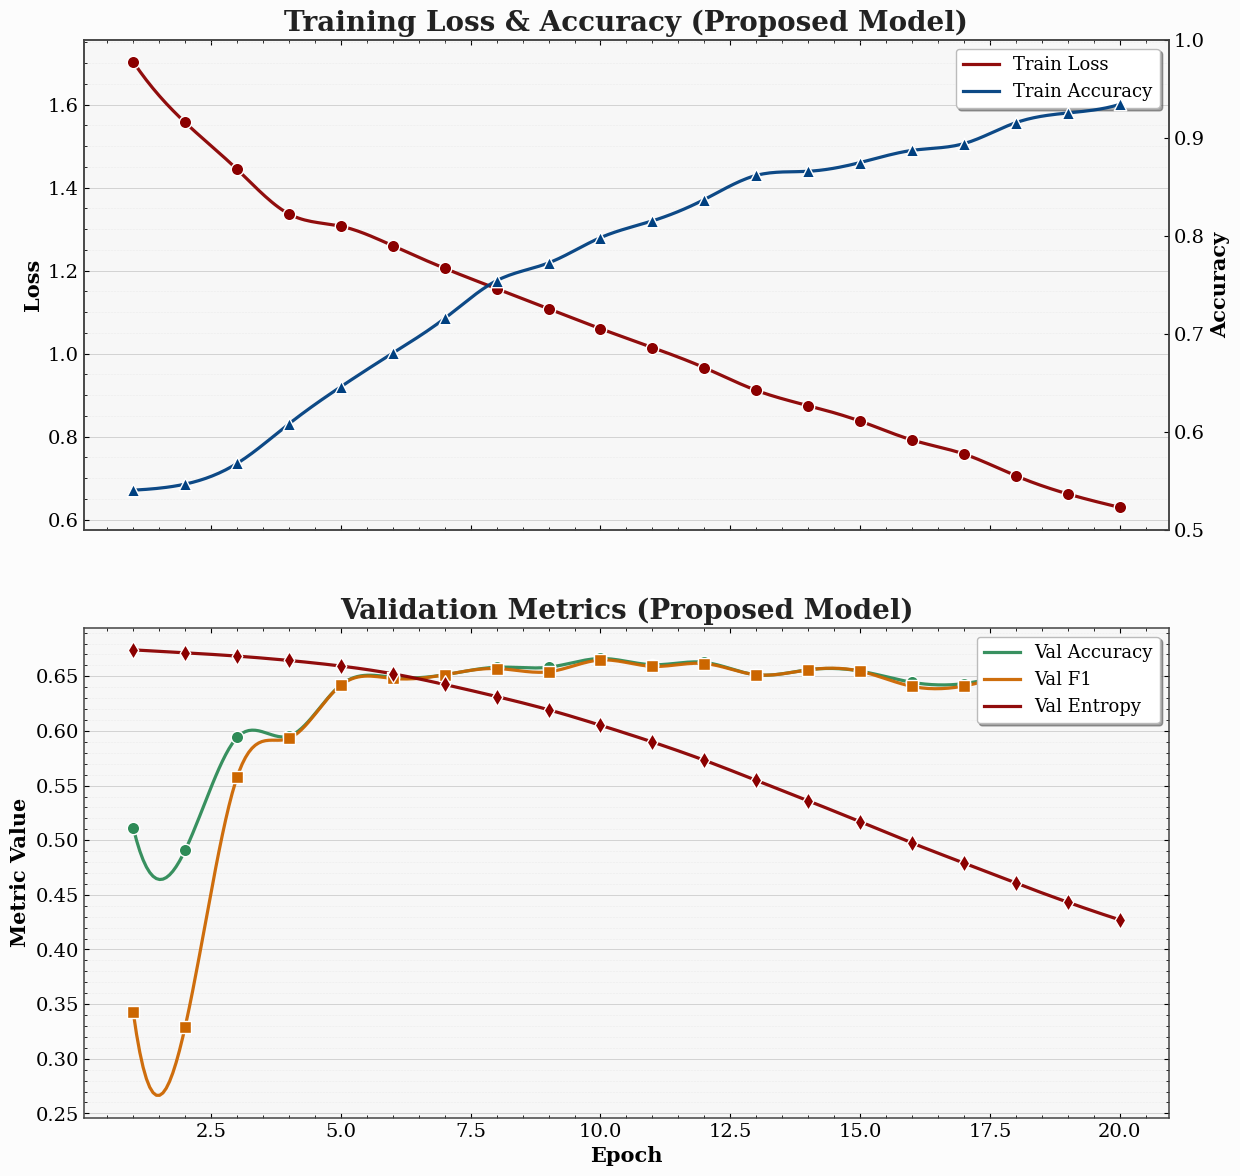
\includegraphics[width=0.7\linewidth]{b_proposed_mnli_stats.png}
    \caption{Balanced - MultiNLI Proposed Model results.}
    \label{fig:r}
\end{figure}


\begin{figure}[H]
    \centering
    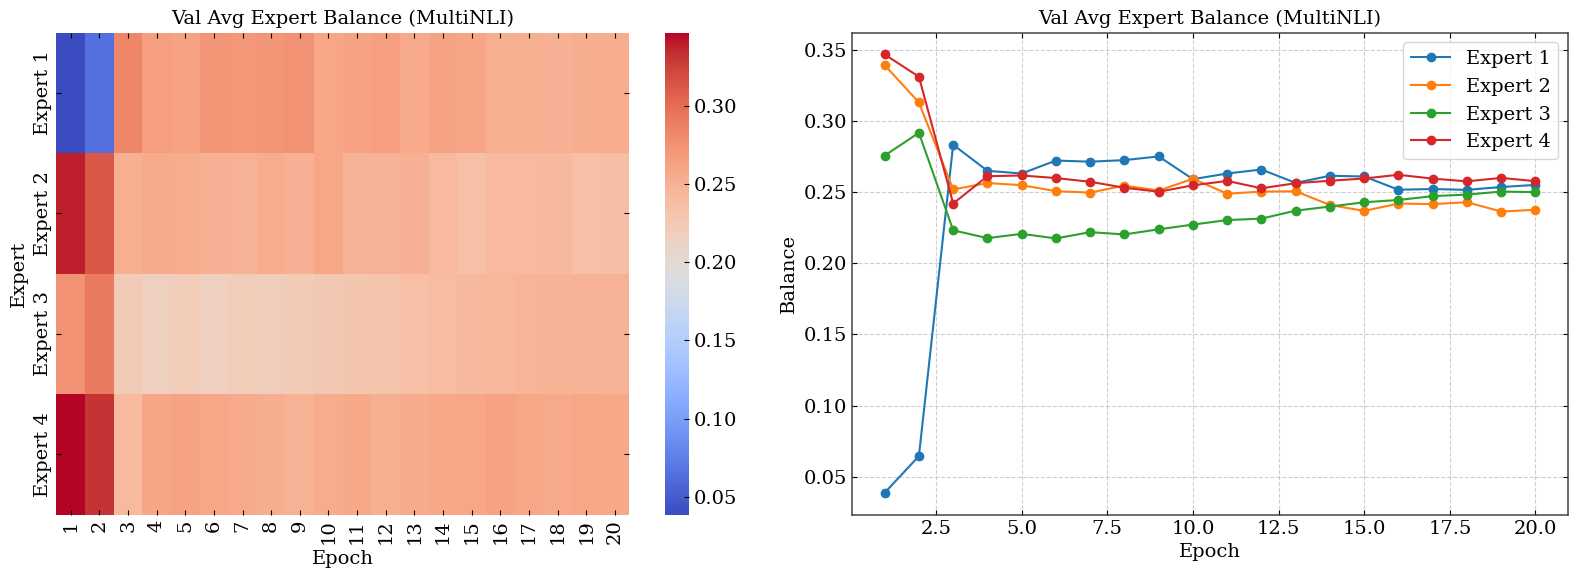
\includegraphics[width=1\linewidth]{b_visuals_mnli.png}
    \caption{Balanced - Average Expert Balance visuals.}
    \label{fig:e}
\end{figure}


\begin{figure}[H]
    \centering
    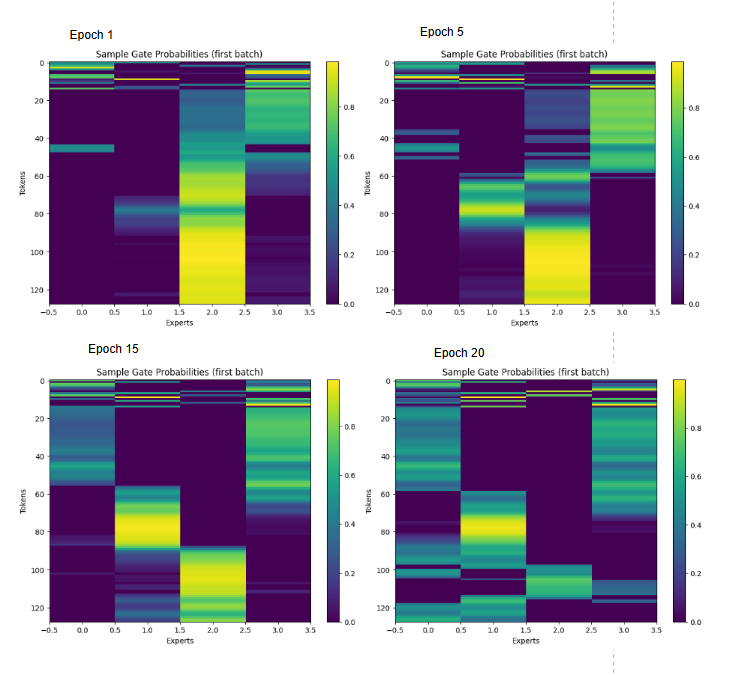
\includegraphics[width=0.7\linewidth]{b_tokens.png}
    \caption{Balanced - Token Gating Probabilities.}
    \label{fig:t}
\end{figure}



\begin{table}[h]
\centering
\small
\setlength{\tabcolsep}{4pt}
\begin{tabular}{c c c c c c c}
\hline
\textbf{Epoch} & \textbf{Train Acc} & \textbf{Train Loss} & \textbf{Val Acc} & \textbf{Val F1} & \textbf{Val Entropy} & \textbf{Val Avg Expert Balance} \\
\hline
1  & 0.5402 & 1.7028 & 0.5115 & 0.3426 & 0.6742 & [0.0387, 0.3391, 0.2756, 0.3466] \\
2  & 0.5464 & 1.5567 & 0.4908 & 0.3292 & 0.6715 & [0.0645, 0.3129, 0.2916, 0.3310] \\
3  & 0.5675 & 1.4439 & 0.5940 & 0.5577 & 0.6685 & [0.2832, 0.2518, 0.2231, 0.2419] \\
4  & 0.6079 & 1.3363 & 0.5952 & 0.5931 & 0.6645 & [0.2649, 0.2563, 0.2176, 0.2611] \\
5  & 0.6458 & 1.3067 & 0.6422 & 0.6419 & 0.6594 & [0.2630, 0.2548, 0.2206, 0.2616] \\
6  & 0.6801 & 1.2596 & 0.6491 & 0.6480 & 0.6523 & [0.2721, 0.2506, 0.2174, 0.2598] \\
7  & 0.7155 & 1.2053 & 0.6514 & 0.6514 & 0.6425 & [0.2713, 0.2496, 0.2218, 0.2572] \\
8  & 0.7540 & 1.1563 & 0.6583 & 0.6571 & 0.6315 & [0.2724, 0.2545, 0.2202, 0.2530] \\
9  & 0.7721 & 1.1080 & 0.6583 & 0.6541 & 0.6194 & [0.2750, 0.2510, 0.2238, 0.2502] \\
10 & 0.7979 & 1.0599 & 0.6663 & 0.6649 & 0.6052 & [0.2590, 0.2593, 0.2271, 0.2547] \\
11 & 0.8150 & 1.0144 & 0.6606 & 0.6591 & 0.5899 & [0.2630, 0.2488, 0.2303, 0.2578] \\
12 & 0.8368 & 0.9659 & 0.6628 & 0.6617 & 0.5732 & [0.2658, 0.2503, 0.2313, 0.2526] \\
13 & 0.8614 & 0.9113 & 0.6514 & 0.6514 & 0.5548 & [0.2564, 0.2505, 0.2369, 0.2562] \\
14 & 0.8656 & 0.8744 & 0.6560 & 0.6559 & 0.5361 & [0.2614, 0.2409, 0.2398, 0.2579] \\
15 & 0.8745 & 0.8372 & 0.6548 & 0.6547 & 0.5170 & [0.2609, 0.2367, 0.2428, 0.2595] \\
16 & 0.8869 & 0.7917 & 0.6445 & 0.6408 & 0.4975 & [0.2516, 0.2419, 0.2444, 0.2621] \\
17 & 0.8938 & 0.7579 & 0.6433 & 0.6411 & 0.4791 & [0.2521, 0.2415, 0.2471, 0.2594] \\
18 & 0.9152 & 0.7054 & 0.6560 & 0.6559 & 0.4608 & [0.2515, 0.2428, 0.2482, 0.2575] \\
19 & 0.9251 & 0.6617 & 0.6720 & 0.6720 & 0.4433 & [0.2535, 0.2363, 0.2503, 0.2599] \\
20 & 0.9338 & 0.6294 & 0.6468 & 0.6448 & 0.4272 & [0.2550, 0.2375, 0.2499, 0.2576] \\
\hline
\end{tabular}
\caption{Balanced - MultiNLI Proposed Model metrics per epoch.}
\label{tab:metrics2}
\end{table}

\vspace{2cm}
\noindent
\subsubsection{Specialized Proposed Model}


\begin{figure}[H]
    \centering
    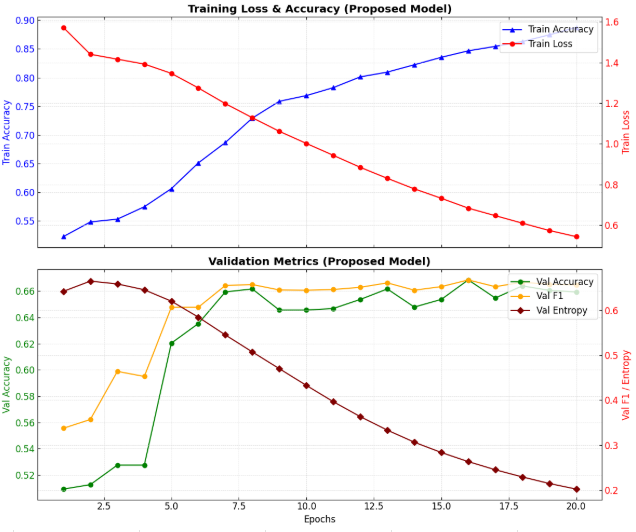
\includegraphics[width=0.74\linewidth]{s_graphs.png}
    \caption{Specialized - MultiNLI Proposed Model results.}
    \label{fig:o}
\end{figure}


\begin{figure}[H]
    \centering
    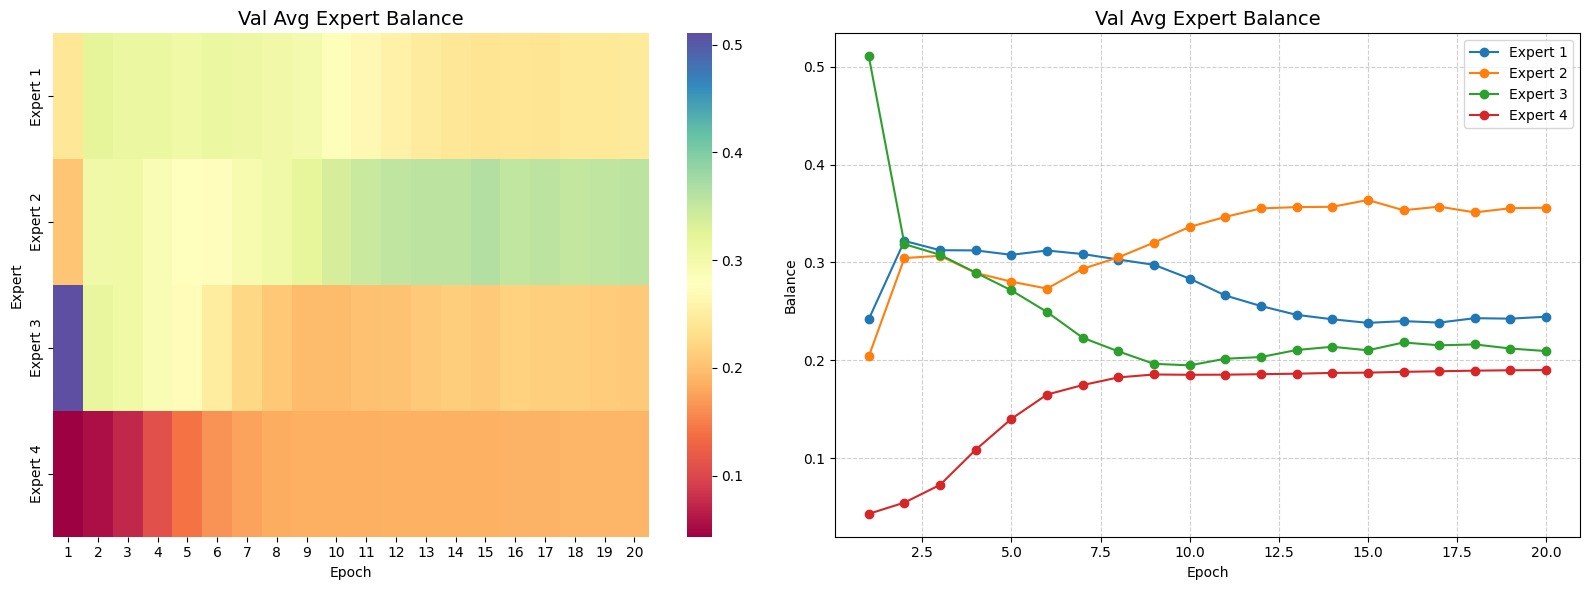
\includegraphics[width=1\linewidth]{s_visuals.png}
    \caption{Specialized - Average Expert Balance visuals.}
    \label{fig:i}
\end{figure}


\begin{figure}[H]
    \centering
    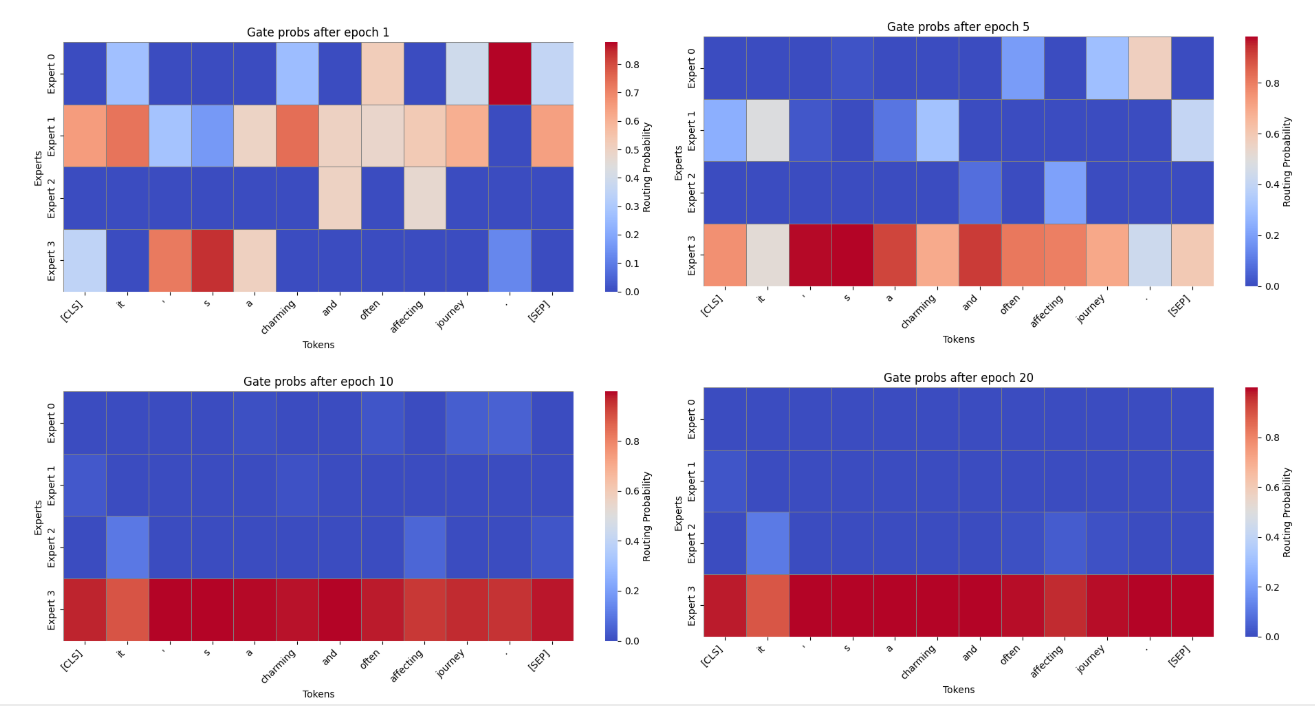
\includegraphics[width=0.7\linewidth]{s_tokens.png}
    \caption{Specialized - Token Gating Probabilities.}
    \label{fig:z}
\end{figure}



\begin{table}[ht!]
\centering
\small
\scriptsize
\setlength{\tabcolsep}{3pt}
\renewcommand{\arraystretch}{1.1}
\begin{tabular}{c|ccccc|c}
\hline
\textbf{Epoch} & \textbf{Train Loss} & \textbf{Train Acc} & \textbf{Val Acc} & \textbf{Val F1} & \textbf{Val Entropy} & \textbf{Val Avg Experts} \\
\hline
1 & 1.5728 & 0.5228 & 0.5092 & 0.3374 & 0.6424 & [0.2421, 0.2041, 0.5106, 0.0433] \\
2 & 1.4406 & 0.5484 & 0.5126 & 0.3570 & 0.6653 & [0.3220, 0.3045, 0.3187, 0.0548] \\
3 & 1.4165 & 0.5533 & 0.5275 & 0.4641 & 0.6590 & [0.3125, 0.3068, 0.3078, 0.0729] \\
4 & 1.3926 & 0.5749 & 0.5275 & 0.4529 & 0.6459 & [0.3123, 0.2893, 0.2896, 0.1088] \\
5 & 1.3467 & 0.6064 & 0.6204 & 0.6070 & 0.6206 & [0.3078, 0.2804, 0.2715, 0.1403] \\
6 & 1.2750 & 0.6513 & 0.6353 & 0.6070 & 0.5850 & [0.3122, 0.2733, 0.2494, 0.1651] \\
7 & 1.1979 & 0.6868 & 0.6594 & 0.6555 & 0.5454 & [0.3086, 0.2935, 0.2231, 0.1748] \\
8 & 1.1285 & 0.7294 & 0.6617 & 0.6576 & 0.5075 & [0.3030, 0.3052, 0.2092, 0.1826] \\
9 & 1.0615 & 0.7587 & 0.6456 & 0.6455 & 0.4702 & [0.2976, 0.3203, 0.1965, 0.1856] \\
10 & 1.0020 & 0.7686 & 0.6456 & 0.6449 & 0.4330 & [0.2835, 0.3363, 0.1949, 0.1853] \\
11 & 0.9433 & 0.7825 & 0.6468 & 0.6465 & 0.3966 & [0.2663, 0.3465, 0.2017, 0.1854] \\
12 & 0.8842 & 0.8013 & 0.6537 & 0.6514 & 0.3633 & [0.2555, 0.3552, 0.2034, 0.1859] \\
13 & 0.8301 & 0.8095 & 0.6617 & 0.6614 & 0.3333 & [0.2465, 0.3565, 0.2106, 0.1864] \\
14 & 0.7783 & 0.8224 & 0.6479 & 0.6450 & 0.3064 & [0.2420, 0.3568, 0.2139, 0.1872] \\
15 & 0.7319 & 0.8353 & 0.6537 & 0.6529 & 0.2834 & [0.2383, 0.3638, 0.2103, 0.1875] \\
16 & 0.6832 & 0.8467 & 0.6686 & 0.6680 & 0.2631 & [0.2401, 0.3533, 0.2183, 0.1883] \\
17 & 0.6464 & 0.8544 & 0.6548 & 0.6528 & 0.2450 & [0.2386, 0.3570, 0.2154, 0.1889] \\
18 & 0.6094 & 0.8628 & 0.6640 & 0.6629 & 0.2290 & [0.2431, 0.3511, 0.2163, 0.1895] \\
19 & 0.5734 & 0.8745 & 0.6606 & 0.6580 & 0.2144 & [0.2426, 0.3554, 0.2121, 0.1899] \\
20 & 0.5430 & 0.8874 & 0.6594 & 0.6570 & 0.2019 & [0.2446, 0.3559, 0.2095, 0.1901] \\
\hline
\end{tabular}
\caption{Specialized - MultiNLI Proposed Model metrics per epoch.}
\label{tab:metrics}
\end{table}




\vspace{6cm}
\noindent
\subsubsection{Vanilla Transformer}


The Vanilla Transformer classifier maps input tokens to embeddings, adds sinusoidal positional encodings, passes them through a stack of 2 Transformer encoder layers with multi-head self-attention, feedforward networks, residual connections, and layer normalization, then averages the token representations, applies dropout, and uses a linear layer to predict the three output classes. The model was run with the same configurations as proposed. 

\begin{figure}[H]
    \centering
    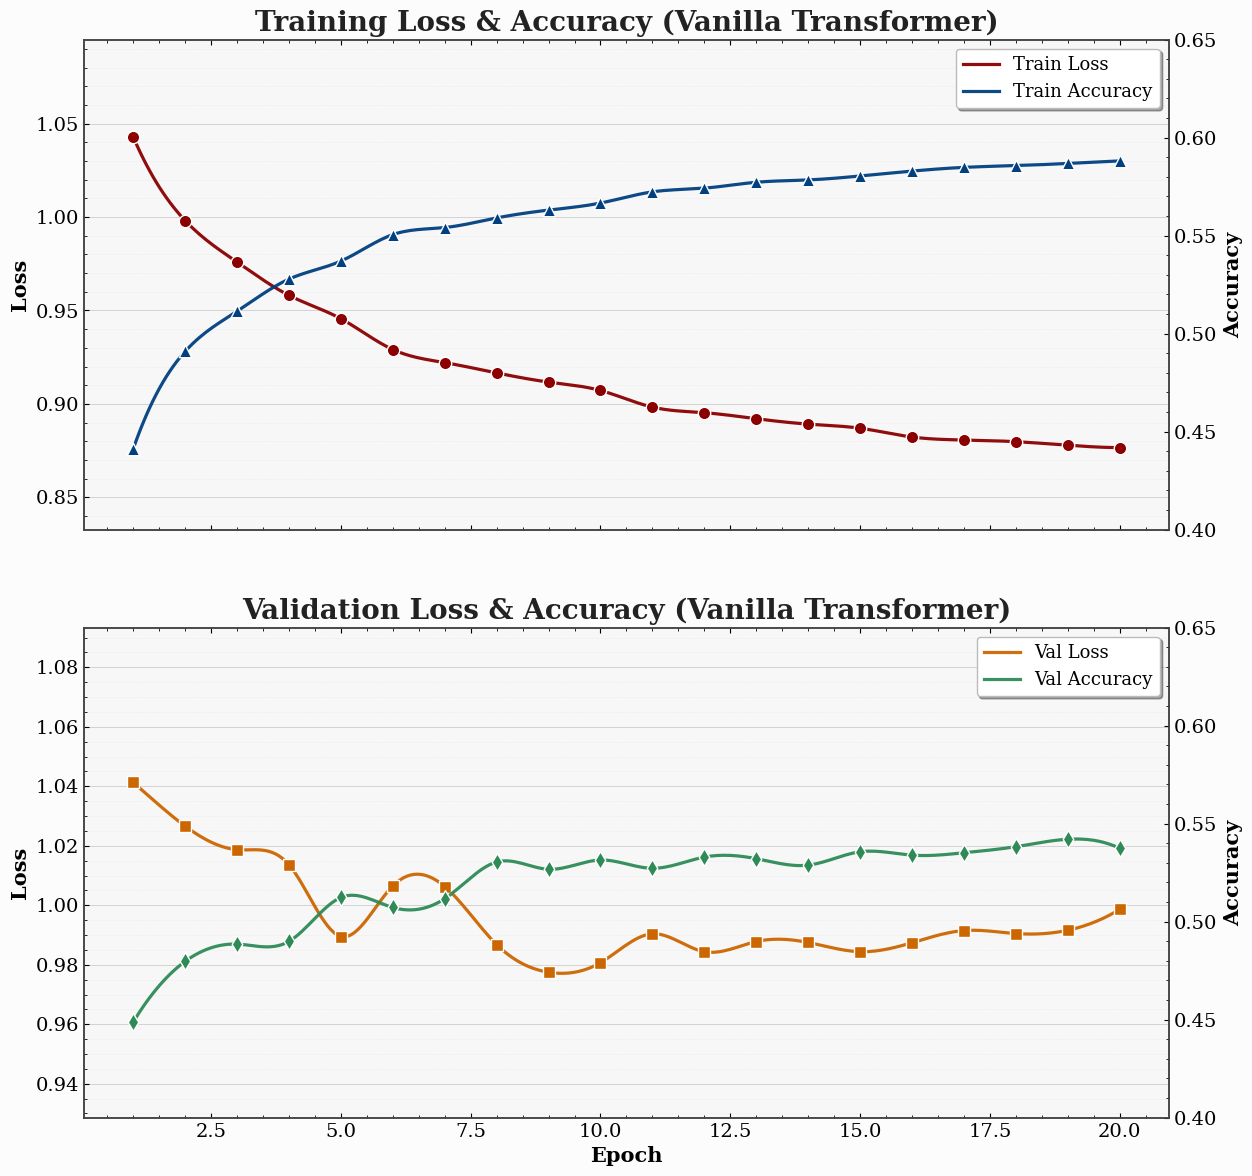
\includegraphics[width=0.7\linewidth]{b_mnli_van_trans.png}
    \caption{MultiNLI Vanilla Transformer results.}
    \label{fig:a}
\end{figure}



\begin{table}[ht]
\centering
\resizebox{\textwidth}{!}{%
\begin{tabular}{c c c c c c c c c}
\toprule
\textbf{Epoch} & \textbf{Train Loss} & \textbf{Train Acc} & \textbf{Train Time (s)} & \textbf{Val Loss} & \textbf{Val Acc} & \textbf{Val Time (s)} & \textbf{Batch Infer Latency (ms)} & \textbf{GPU Mem Allocated (MB)} \\
\midrule
1 & 1.0428 & 0.4412 & 146.95 & 1.0413 & 0.4488 & 1.23 & 1.9 & 81.98 \\
2 & 0.9981 & 0.4909 & 154.75 & 1.0266 & 0.4797 & 1.06 & 1.8 & 81.98 \\
3 & 0.9759 & 0.5114 & 144.8 & 1.0187 & 0.4885 & 1.06 & 1.79 & 81.98 \\
4 & 0.9581 & 0.5278 & 137.3 & 1.0136 & 0.4899 & 1.23 & 1.88 & 81.98 \\
5 & 0.9456 & 0.537 & 137.41 & 0.9895 & 0.5123 & 1.07 & 1.81 & 81.98 \\
6 & 0.9291 & 0.5505 & 137.81 & 1.0065 & 0.5072 & 1.23 & 1.85 & 81.98 \\
7 & 0.9221 & 0.5541 & 137.33 & 1.0063 & 0.5117 & 1.06 & 1.79 & 81.98 \\
8 & 0.9166 & 0.559 & 137.39 & 0.9868 & 0.5304 & 1.06 & 1.79 & 81.98 \\
9 & 0.9117 & 0.563 & 137.23 & 0.9775 & 0.5267 & 1.06 & 1.8 & 81.98 \\
10 & 0.9072 & 0.5666 & 137.14 & 0.9807 & 0.5314 & 1.06 & 1.79 & 81.98 \\
11 & 0.8983 & 0.5723 & 136.74 & 0.9904 & 0.5272 & 1.28 & 1.87 & 81.98 \\
12 & 0.8953 & 0.5742 & 136.96 & 0.9844 & 0.5329 & 1.06 & 1.79 & 81.98 \\
13 & 0.8921 & 0.5772 & 137.82 & 0.9878 & 0.5321 & 1.06 & 1.78 & 81.98 \\
14 & 0.8892 & 0.5784 & 136.77 & 0.9875 & 0.5288 & 1.06 & 1.8 & 81.98 \\
15 & 0.887 & 0.5804 & 136.64 & 0.9844 & 0.5356 & 1.06 & 1.79 & 81.98 \\
16 & 0.8823 & 0.5829 & 136.72 & 0.9874 & 0.5339 & 1.31 & 1.9 & 81.98 \\
17 & 0.8807 & 0.5848 & 137.43 & 0.9915 & 0.5351 & 1.06 & 1.79 & 81.98 \\
18 & 0.8798 & 0.5857 & 136.93 & 0.9905 & 0.5382 & 1.16 & 1.85 & 81.98 \\
19 & 0.8779 & 0.5868 & 138.15 & 0.9916 & 0.542 & 1.06 & 1.79 & 81.98 \\
20 & 0.8766 & 0.5881 & 139.37 & 0.9986 & 0.5374 & 1.26 & 1.88 & 81.98 \\
\bottomrule
\end{tabular}%
}
\caption{MultiNLI  Vanilla Transformer metrics per epoch.}
\end{table}

\subsubsection{Analysis}
The proposed modular Transformer (MT) outperforms the vanilla Transformer on MultiNLI. Across 20 epochs, MT achieves mean validation accuracy of 0.6333 (std $\approx 0.0482$) versus 0.5185 (std $\approx 0.0238$) for the baseline, peaking at 0.6720 at epoch 19 (vs. 0.5240), an absolute improvement of $+0.13$. Training accuracy is higher (0.9338 vs. 0.5881), indicating that MT converts its larger parameter set into greater effective capacity. This gain comes at the cost of higher memory usage: the vanilla model requires 82 MB, while MT consumes multiple times more to store and update experts. This reflects a capacity–memory trade-off: MT offers higher accuracy when hardware allows; in constrained settings, quantization, sparse expert loading, or offloading can reduce memory with limited performance loss.

\vspace{2pt}
\noindent \textbf{Balanced Routing} \vspace{1pt} \
Balanced routing makes full use of the added parameters. The gating distribution shifts from a skewed allocation at epoch 1 ([0.0387, 0.3391, 0.2756, 0.3466]) to nearly uniform by epoch 20 ([0.2550, 0.2375, 0.2499, 0.2576]); $\ell_2$ distance to uniform drops by $\approx 0.235$, and KL-divergence falls from 0.1713 to 0.00048. Uniform expert usage correlates with better generalization (Pearson $\rho \approx -0.92$ between skew magnitude and validation accuracy), prevents expert collapse, distributes gradients evenly, and stabilizes optimization. Balanced routing is especially useful in multi-domain inference, reducing domain bias and avoiding bottlenecks from overused experts.

\vspace{1pt}
\noindent \textbf{Specialization} \vspace{1pt} \
Specialization allows experts to develop complementary skills. Early skew patterns indicate niche formation, and prediction entropy decreases over training (0.6742 $\rightarrow$ 0.4272), showing that experts become more decisive. This diversity drives MT’s higher validation ceiling (0.6720 vs. 0.5420), as experts capture distinct linguistic features such as negation, coreference, or domain-specific vocabulary. Specialization increases capacity and can cause overfitting; at epoch 20, the train–validation gap is 28.7 points. It is most effective in heterogeneous data environments (e.g., legal vs. medical text), and overfitting can be mitigated using balancing, regularization (weight decay, dropout, early stopping), or memory-efficient strategies (quantized experts, disk-backed modules, dynamic expert loading).




\section{Conclusion}
The modular Transformer shows clear improvements over a vanilla baseline, providing richer token-level representations and more specialized processing. While results on MultiNLI demonstrate better accuracy and generalization, future work should evaluate the model on additional benchmarks such as SNLI, SQuAD, CoQA, GLUE, and multimodal datasets like VQA and MS COCO to test broader applicability.

\section{References}
[1] Ashish Vaswani, Noam Shazeer, Niki Parmar, Jakob Uszkoreit, Llion Jones, Aidan N. Gomez, Łukasz Kaiser, and Illia Polosukhin. Attention is All You Need. 2017. https://arxiv.org/abs/1706.03762

\vspace{7pt}
\noindent
[2] Noam Shazeer, Azalia Mirhoseini, Krzysztof Maziarz, Andy Davis, Quoc Le, Geoffrey Hinton, and Jeff Dean. Outrageously Large Neural Networks: The Sparsely-Gated Mixture-of-Experts Layer. 2017. https://arxiv.org/abs/1701.06538

\vspace{7pt}
\noindent
[3]
Xun Wu, Shaohan Huang, and Furu Wei. Mixture of LoRA Experts (MoLE). 2024. 
https://arxiv.org/abs/2404.13628


\vspace{7pt}
\noindent
[4]
Ethan Perez, Florian Strub, Harm de Vries, Vincent Dumoulin, and Aaron Courville. FiLM: Visual Reasoning with a General Conditioning Layer. 2017. https://arxiv.org/abs/1709.07871


\end{document}
